\chapter{Les cycles biogéochimiques}\label{ch:b2:biogeochemical-cycles}

En mars 1958, un jeune chimiste nommé Charles Keeling mit en marche un
analyseur de gaz à infrarouge sur le versant nord du Mauna Loa, à Hawaï,
à trois kilomètres et demi au-dessus du Pacifique, là où l'air est aussi
bien mélangé que l'air peut l'être. Il s'attendait à mesurer une
constante~; au bout d'un an, il obtenait une courbe en dents de scie ---
le dioxyde de carbone augmentant chaque hiver et diminuant chaque été, au
rythme de la respiration des forêts de l'hémisphère nord --- et, au bout
de quelques années, une pente sous les dents de scie qui ne s'est jamais
interrompue depuis. La \omterm{prop:b2:biogeochemical-cycles:carbon}{courbe de Keeling} est la respiration de la
biosphère vue de l'extérieur, avec une courbe de fièvre tracée par-dessus.
Ce chapitre traite des cycles qu'enregistre cette courbe~: où sont
stockés le carbone, l'azote, le phosphore et le soufre des êtres vivants,
à quelle vitesse ils passent d'un \omterm{def:b2:biogeochemical-cycles:reservoir}{réservoir} à l'autre, ce qui fixe ces
vitesses --- pour la plupart les métabolismes du
\cref{ch:b2:microbial-metabolism} --- et ce qu'une seule espèce a fait à
chaque cycle en deux cents ans.

\section{Réservoirs, flux et temps de résidence}

\begin{definition}[Réservoir, flux, temps de résidence]\label{def:b2:biogeochemical-cycles:reservoir}
\index{reservoir@réservoir}\index{flux}\index{temps de residence@temps de résidence}\index{etat stationnaire@état stationnaire}\index{cycle biogeochimique@cycle biogéochimique}
Un \emph{cycle biogéochimique} est le déplacement d'un élément entre des
\emph{réservoirs} (l'atmosphère, l'océan, les sols, la biomasse vivante,
les roches) par des \emph{flux} mesurés en masse par an. Un réservoir de
masse $M$ dont le flux sortant total vaut $F$ a un \emph{temps de
résidence} $\tau = M/F$, la durée moyenne qu'y passe un atome~; à
l'\emph{état stationnaire}, le flux entrant égale le flux sortant et $M$
est constante. Les cycles sont couplés par la stœchiométrie du vivant ---
le \emph{rapport de Redfield} du plancton marin, $\mathrm{C:N:P} =
106:16:1$ en atomes --- si bien que l'apport de l'élément le plus rare
fixe la vitesse à laquelle tous les autres sont absorbés.
\end{definition}

\begin{theorem}[Le modèle à un compartiment]\label{thm:b2:biogeochemical-cycles:box}
\index{modele a un compartiment@modèle à un compartiment}\index{temps de relaxation}
Si un \omterm{def:b2:biogeochemical-cycles:reservoir}{réservoir} perd son contenu à une vitesse proportionnelle à ce qu'il
contient, $F_{\text{out}} = M/\tau$, et reçoit un \omterm{def:b2:biogeochemical-cycles:reservoir}{flux} entrant constant
$F_{\text{in}}$, alors
\[
\frac{\mathrm{d}M}{\mathrm{d}t} = F_{\text{in}} - \frac{M}{\tau},
\qquad
M(t) = M^{*} + (M_0 - M^{*})\,e^{-t/\tau}, \qquad M^{*} = F_{\text{in}}\tau :
\]
le \omterm{def:b2:biogeochemical-cycles:reservoir}{réservoir} tend vers un \omterm{def:b2:biogeochemical-cycles:reservoir}{état stationnaire} proportionnel à son apport,
avec le \omterm{def:b2:biogeochemical-cycles:reservoir}{temps de résidence} comme constante de temps. Une augmentation en
échelon de l'apport élève l'\omterm{def:b2:biogeochemical-cycles:reservoir}{état stationnaire} en proportion et le
\omterm{def:b2:biogeochemical-cycles:reservoir}{réservoir} suit en quelques $\tau$~: un compartiment dont le \omterm{def:b2:biogeochemical-cycles:reservoir}{temps de
résidence} se compte en jours (l'ammoniac atmosphérique, le nitrate d'un
lac au printemps) suit ses sources~; un compartiment dont le \omterm{def:b2:biogeochemical-cycles:reservoir}{temps de
résidence} se compte en siècles (le carbone de l'océan profond, la matière
organique des sols) les intègre, et la perturbation d'un compartiment
lent survit à la perturbation qui l'a causée.
\end{theorem}
\begin{proof}
L'équation est linéaire à coefficients constants~: l'\omterm{def:b2:biogeochemical-cycles:reservoir}{état stationnaire}
$M^{*}$ annule le second membre, et l'écart $m = M - M^{*}$
obéit à $\dot m = -m/\tau$, donc $m = m_0 e^{-t/\tau}$. Si un \omterm{def:b2:biogeochemical-cycles:reservoir}{réservoir}
a plusieurs \omterm{def:b2:biogeochemical-cycles:reservoir}{flux} sortants, $\tau$ est fixé par leur somme, $1/\tau = \sum_i
1/\tau_i$~: le puits le plus rapide domine.
\end{proof}

\section{Le cycle du carbone}

\begin{proposition}[Le bilan du carbone]\label{prop:b2:biogeochemical-cycles:carbon}
\index{cycle du carbone}\index{fraction atmospherique@fraction atmosphérique}\index{puits de carbone}\index{courbe de Keeling}
En gigatonnes de carbone (\unit{GtC}, $10^{12}$~kg), les principaux
\omterm{def:b2:biogeochemical-cycles:reservoir}{réservoirs} sont l'atmosphère (environ 880 dans les années 2020, 590
avant l'industrie), les plantes terrestres (450), les sols (1700),
l'océan superficiel (900), l'océan profond (\num{37000}) et les roches
sédimentaires
(\num{e8})~; les combustibles fossiles sont la fraction de ces dernières
que l'industrie peut atteindre, quelque \num{5000}. Les \omterm{def:b2:biogeochemical-cycles:reservoir}{flux} naturels sont
importants et presque équilibrés~: la photosynthèse terrestre prélève
environ 120 par an, que la respiration et la décomposition restituent~; la
surface de l'océan échange avec l'air environ 80 dans chaque sens. Le \omterm{def:b2:biogeochemical-cycles:reservoir}{flux}
humain est faible en comparaison --- quelque 10 par an issus des
combustibles fossiles et 1 de la déforestation --- mais à sens unique, et
l'atmosphère en a conservé \emph{environ \qty{45}{\%}} (la \emph{\omterm{prop:b2:biogeochemical-cycles:carbon}{fraction
atmosphérique}}), l'océan en prenant un quart et les terres, fertilisées
par le surplus de
$\mathrm{CO_2}$, le reste. Une partie par million de $\mathrm{CO_2}$ atmosphérique représente
\qty{2.13}{GtC}~; la concentration est passée de 280 à \num{315}~ppm
entre 1750 et 1958, et de 315 à plus de \num{420} entre 1958 et les
années 2020, avec actuellement \qty{2.5}{ppm} par an. Le \omterm{def:b2:biogeochemical-cycles:reservoir}{temps de
résidence} d'une molécule de $\mathrm{CO_2}$ dans l'air, $880/200 \approx 4$ ans,
est court~; la durée de vie de l'\emph{excédent}, fixée par le lent
mélange avec l'océan profond et par l'altération plus lente encore des
roches, se compte en siècles ou en millénaires --- un cinquième de ce qui
est émis aujourd'hui sera encore dans l'air dans dix mille ans.
\end{proposition}
\begin{proof}[Faits expérimentaux]
Trois signatures montrent que le carbone ajouté est fossile. Ses
isotopes~: le carbone fossile ne contient pas de $\mathrm{{}^{14}C}$ (il s'est
désintégré il y a des millions d'années) et il est appauvri en $\mathrm{{}^{13}C}$ comme tout carbone
végétal, et l'atmosphère perd les deux --- l'effet Suess, mesuré dans les
cernes des arbres depuis les années 1950. Son oxygène~: l'$\mathrm{O_2}$ de
l'atmosphère diminue en proportion, selon la stœchiométrie de la
combustion, comme l'a montré le fils de Keeling dans les années 1990, ce
qu'une source volcanique ou océanique ne produirait pas. Sa
comptabilité~: la somme du charbon, du pétrole et du gaz vendus, convertie
en carbone, dépasse d'un facteur deux l'augmentation dans l'air, et la
moitié manquante se retrouve dans l'augmentation du carbone inorganique
dissous de l'océan et la baisse de son pH, ainsi que dans le puits
terrestre. Les dents de scie saisonnières, plus marquées à Barrow, en
Alaska, qu'au Mauna Loa et presque absentes au pôle Sud, sont
l'absorption estivale et le rejet hivernal des forêts du Nord --- une
mesure directe de la respiration de la biosphère.
\end{proof}

\begin{omfigure}
\begin{tikzpicture}
\begin{axis}[
  width=0.9\linewidth, height=6cm,
  axis x line=bottom, axis y line=left,
  xmin=1955, xmax=2026, ymin=300, ymax=430,
  xlabel={année}, ylabel={$\mathrm{CO_2}$ (ppm), moyenne annuelle au Mauna Loa},
  xlabel style={font=\small, at={(axis description cs:0.5,-0.13)}, anchor=north},
  ylabel style={font=\small},
  tick label style={font=\small}, xtick={1960,1970,1980,1990,2000,2010,2020}, ytick={300,325,350,375,400,425},
  scaled x ticks=false, x tick label style={/pgf/number format/1000 sep=},
  clip=false,
]
\addplot[very thick, omDef, mark=*, mark size=1pt] coordinates {
(1959,316.0) (1962,318.5) (1965,320.0) (1968,323.0) (1971,326.3) (1974,330.2) (1977,333.8) (1980,338.8) (1983,342.8) (1986,347.2) (1989,353.1) (1992,356.4) (1995,360.8) (1998,366.7) (2001,371.1) (2004,377.5) (2007,383.8) (2010,389.9) (2013,396.5) (2016,404.2) (2019,411.4) (2022,418.5) (2024,424.6)};
\node[font=\scriptsize, anchor=north west, align=left] at (axis cs:1958,425) {années 1960~: \qty{+0.9}{ppm/yr}\\années 2010~: \qty{+2.4}{ppm/yr}};
\node[font=\scriptsize, anchor=west, align=left] at (axis cs:1990,320) {niveau préindustriel~: \qty{280}{ppm}~;\\des dents de scie annuelles\\de $\pm\qty{3}{ppm}$ s'y superposent};
\end{axis}
\end{tikzpicture}

{\small La \omterm{prop:b2:biogeochemical-cycles:carbon}{courbe de Keeling}~: moyenne annuelle du dioxyde de carbone de
l'air au Mauna Loa depuis 1959. La pente a presque triplé~; les dents de
scie saisonnières qui s'y superposent, invisibles à cette échelle, sont
la photosynthèse estivale de l'hémisphère nord.}
\end{omfigure}

\begin{omfigure}
\begin{tikzpicture}[every node/.style={font=\scriptsize}, >=stealth, box/.style={draw, rounded corners, minimum width=2.2cm, minimum height=0.9cm, align=center, fill=#1}]
  \node[box=omDef!15] (atm) at (0,3) {atmosphère\\880};
  \node[box=omThm!15] (veg) at (-4.4,0.6) {plantes terrestres 450\\sols 1700};
  \node[box=omProp!15] (surf) at (4.4,0.6) {océan superficiel\\900};
  \node[box=omProp!25] (deep) at (4.4,-1.6) {océan profond\\37\,000};
  \node[box=gray!20] (rock) at (0,-1.6) {roches et combustibles fossiles\\$10^{8}$~; accessibles $\sim 5000$};
  \draw[->, thick] ([xshift=-2mm]atm.south west) -- node[above left, pos=0.45] {120 photosynthèse} ([xshift=-4mm]veg.north);
  \draw[->, thick] ([xshift=5mm]veg.north) -- ([xshift=-2mm]atm.south); \node[anchor=north east] at (-0.4,1.5) {119 respiration, feux};
  \draw[->, thick] ([xshift=2mm]atm.south east) -- node[above right, pos=0.45] {80 dissolution} ([xshift=4mm]surf.north);
  \draw[->, thick] ([xshift=-5mm]surf.north) -- ([xshift=2mm]atm.south); \node[anchor=north west] at (0.4,1.5) {78 dégazage};
  \draw[<->, thick] (surf) -- node[right] {$\sim 100$ mélange, chute} (deep);
  \draw[->, very thick, omExo!80!black] (rock.north) -- node[left, align=right, pos=0.4] {10 combustibles fossiles\\ + 1 usage des terres} (atm.south);
  \node[align=left, anchor=west] at (7.0,3.2) {flux en \unit{GtC/yr},\\ stocks en \unit{GtC}\\[2pt] sur les 11 émises~:\\ 5 restent dans l'air,\\ 3 vont aux terres,\\ 3 vont à l'océan};
\end{tikzpicture}

{\small Le \omterm{prop:b2:biogeochemical-cycles:carbon}{cycle du carbone} en chiffres ronds. Les échanges naturels
représentent dix fois le \omterm{def:b2:biogeochemical-cycles:reservoir}{flux} humain, mais ils se compensent presque~; le
\omterm{def:b2:biogeochemical-cycles:reservoir}{flux} humain, lui, ne se compense pas.}
\end{omfigure}

\begin{omfigure}
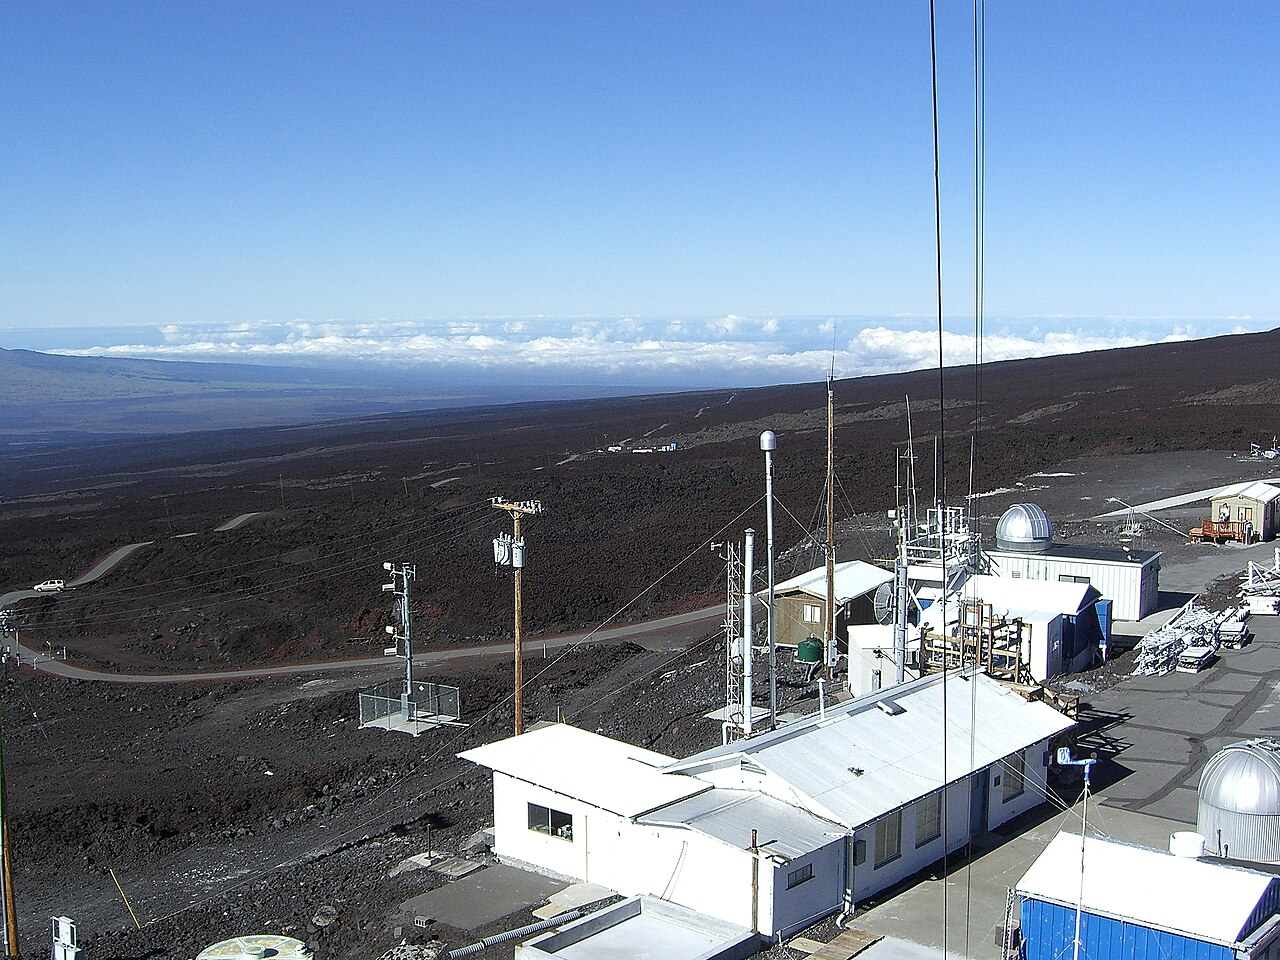
\includegraphics[width=0.56\linewidth]{images/book4/mauna-loa.jpg}\hspace{0.03\linewidth}
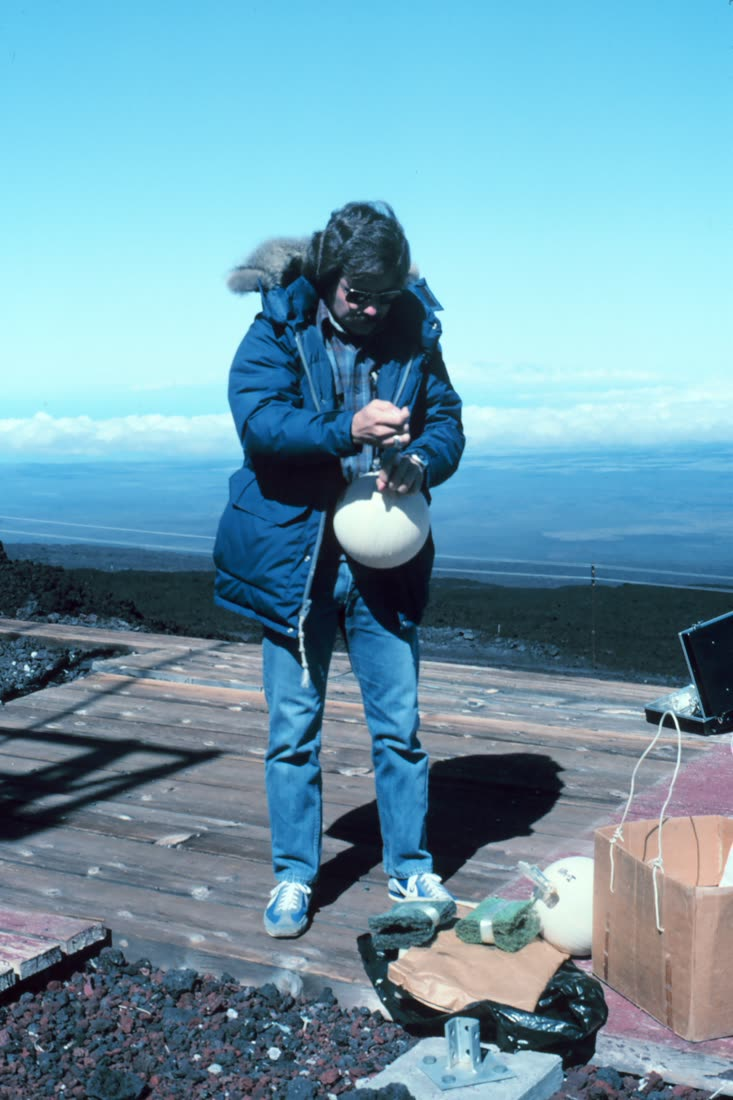
\includegraphics[width=0.33\linewidth]{images/book4/keeling-flask.jpg}

{\small Là où la courbe est tracée. À gauche~: l'observatoire du versant
nord du Mauna Loa, à \qty{3400}{m} d'altitude, au-dessus de l'inversion
des alizés qui maintient en contrebas l'air propre de l'île. À droite~:
un prélèvement en flacon effectué en 1982~; des flacons comme ceux-ci,
analysés en Californie, servent à vérifier l'analyseur continu et sont
remplis dans des stations allant de l'Alaska au pôle Sud.}
\end{omfigure}

\section{Le cycle de l'azote}

\begin{proposition}[Le cycle de l'azote]\label{prop:b2:biogeochemical-cycles:nitrogen}
\index{cycle de l'azote}\index{fixation de l'azote}\index{nitrification}\index{denitrification@dénitrification}\index{procede Haber--Bosch@procédé Haber--Bosch}\index{anammox}
L'azote est abondant --- l'air contient $4\times 10^{9}$~Tg de
$\mathrm{N_2}$ --- et rare, parce que la triple liaison de $\mathrm{N_2}$ n'est ouverte
que par deux processus~: la foudre (quelques Tg par an) et la
\emph{fixation biologique de l'azote} par des \omterm{def:b2:unicellular-diversity:prokaryote}{procaryotes} possédant la
nitrogénase, quelque 100 Tg par an sur les terres et 100 en mer, au prix
de 16 ATP par $\mathrm{N_2}$. L'azote fixé descend ensuite une échelle
d'oxydoréduction entraînée par des microbes (\cref{ch:b2:microbial-metabolism})~:
\emph{ammonification} de la matière morte en $\mathrm{NH_4^{+}}$~;
\emph{nitrification} de $\mathrm{NH_4^{+}}$ en $\mathrm{NO_2^{-}}$ et $\mathrm{NO_3^{-}}$ par
des \omterm{def:b2:microbial-metabolism:trophic}{chimiolithotrophes} aérobies~; absorption de $\mathrm{NH_4^{+}}$ ou de $\mathrm{NO_3^{-}}$ par les plantes
et leur réduction en groupements amine~; et, là où l'oxygène manque,
\emph{\omterm{def:b2:microbial-metabolism:anaerobic}{dénitrification}} de $\mathrm{NO_3^{-}}$ en $\mathrm{N_2}$ (avec des fuites de $\mathrm{N_2O}$)
et \emph{anammox}, l'oxydation anaérobie de l'ammonium par le
nitrite en $\mathrm{N_2}$, qui ensemble restituent à l'air à peu près autant
que la fixation en prélève. Le \omterm{def:b2:biogeochemical-cycles:reservoir}{temps de résidence} d'un atome d'azote dans
la biosphère est de quelques centaines d'années~; dans l'atmosphère, de $4\times
10^{9}/400 \approx 10^{7}$ ans. Depuis 1913, le procédé \emph{Haber--Bosch}
fixe l'azote industriellement, aujourd'hui environ 120 Tg par an,
et les légumineuses cultivées et la combustion des combustibles fossiles
en ajoutent 60 et 30~: l'activité humaine fixe autant d'azote que
l'ensemble des processus naturels, et nourrit la moitié des êtres humains
vivants.
\end{proposition}

\begin{omfigure}
\begin{tikzpicture}[every node/.style={font=\scriptsize}, >=stealth, box/.style={draw, rounded corners, minimum width=1.9cm, minimum height=0.8cm, align=center, fill=#1}]
  \node[box=omDef!15] (n2) at (0,3.4) {$\mathrm{N_2}$ de l'air\\$4\times 10^{9}$ Tg};
  \node[box=omThm!15] (org) at (-4.6,1.0) {N organique\\plantes, sols, mer};
  \node[box=omProp!15] (nh4) at (-2.2,-0.8) {$\mathrm{NH_4^{+}}$};
  \node[box=omProp!15] (no2) at (2.2,-0.8) {$\mathrm{NO_2^{-}}$};
  \node[box=omProp!15] (no3) at (4.6,1.0) {$\mathrm{NO_3^{-}}$};
  \draw[->, thick] (n2) -- node[above left, align=right] {fixation\\nitrogénase, 200\\Haber--Bosch 120} (org);
  \draw[->, thick] (org.south) -- node[below left] {ammonification} (nh4.north);
  \draw[->, thick] (nh4) -- node[below] {nitrification} (no2);
  \draw[->, thick] (no2) -- node[below right] {nitrification} (no3);
  \draw[->, thick] (no3) to[bend left=18] node[above, pos=0.72] {assimilation} (org);
  \draw[->, thick, omExo!80!black] (no3) -- node[above right, align=left] {dénitrification\\(anoxie), fuite de $\mathrm{N_2O}$} (n2);
  \draw[->, thick, omExo!80!black] (no2) -- node[right, pos=0.55, align=left] {anammox\\(avec $\mathrm{NH_4^{+}}$)} (n2);
  \node[anchor=north, align=center] at (0,-1.5) {flux en Tg N par an~; toutes les étapes sauf l'assimilation et l'ammonification sont assurées par des procaryotes};
\end{tikzpicture}

{\small Le \omterm{prop:b2:biogeochemical-cycles:nitrogen}{cycle de l'azote} comme échelle d'oxydoréduction (les plantes
assimilent l'ammonium aussi bien que le nitrate). La fixation et la
\omterm{def:b2:microbial-metabolism:anaerobic}{dénitrification}, les deux portes de l'atmosphère, sont toutes deux
microbiennes~; la porte industrielle égale désormais la porte naturelle.}
\end{omfigure}

\begin{proof}[Faits expérimentaux]
Dans la forêt expérimentale de Hubbard Brook, dans le New Hampshire, un
bassin versant entier fut coupé à blanc en 1965 et maintenu nu à l'aide
d'herbicides, tandis qu'un bassin voisin était laissé intact, et les
ruisseaux qui drainaient chacun d'eux furent jaugés et analysés pendant
des années. Le bassin mis à nu perdit du nitrate à un rythme soixante
fois supérieur à celui du témoin --- tout le capital azoté du sol, qui
n'était plus absorbé par les plantes, fut nitrifié et lessivé, emportant
avec lui le calcium et le potassium et acidifiant le ruisseau.
L'expérience montra à quel point le cycle est fermé dans une forêt intacte
(quelques kilogrammes d'azote perdus par hectare et par an, contre des
centaines recyclés) et ce qui le rompt.
\end{proof}

\section{Le phosphore et le soufre}

\begin{proposition}[Deux cycles sans gaz rapide]\label{prop:b2:biogeochemical-cycles:ps}
\index{cycle du phosphore}\index{cycle du soufre}\index{eutrophisation}\index{sulfure de dimethyle@sulfure de diméthyle}
Le \emph{phosphore} n'a pas de forme gazeuse. Il entre dans les
écosystèmes par l'altération de l'apatite des roches, quelque 20 Tg par
an sur l'ensemble des terres émergées, est recyclé de nombreuses fois dans
les sols et les lacs
--- un ion phosphate des eaux de surface d'un lac est absorbé en quelques
heures --- et part vers les sédiments, où il demeure pendant les
$10^{8}$ ans d'un cycle des roches. Le vivant est donc économe en
phosphore et limité par le phosphore~: le \omterm{def:b2:biogeochemical-cycles:reservoir}{temps de résidence} dans l'océan
est de quelque
\num{20000} ans, et le phosphate des eaux profondes, remonté par les
upwellings, fixe leur productivité. L'exploitation minière apporte
désormais aux terres agricoles à peu près autant de phosphore que
l'altération en libère, et son ruissellement dans les lacs provoque
l'\emph{eutrophisation}~: une prolifération d'algues, sa décomposition, la
consommation de l'oxygène et la mort des poissons --- les expériences de
Schindler sur des lacs entiers de l'Ontario, dans les années 1970, où l'une
des moitiés d'un lac était fertilisée avec du phosphore et l'autre non,
montrèrent que le phosphore suffit à lui seul à déclencher le phénomène,
et conduisirent à son retrait des détergents.
Le \emph{soufre} a à la fois un cycle des roches (gypse, pyrite) et une
phase gazeuse~: le $\mathrm{SO_2}$ des volcans et du charbon, l'$\mathrm{H_2S}$ des
sédiments anoxiques, et le \emph{\omterm{prop:b2:biogeochemical-cycles:ps}{sulfure de diméthyle}} du plancton marin,
dont les produits d'oxydation ensemencent les nuages au-dessus de l'océan.
La combustion du charbon a triplé le \omterm{def:b2:biogeochemical-cycles:reservoir}{flux} de soufre vers l'air au
\textsc{xx}\textsuperscript{e} siècle et donné à l'Europe et à l'Amérique du Nord
leurs pluies acides~; les épurateurs de fumées l'ont fait reculer en
quelques décennies, le \omterm{def:b2:biogeochemical-cycles:reservoir}{temps de résidence} du soufre dans l'air n'étant
que de quelques jours.
\end{proposition}

\begin{omfigure}
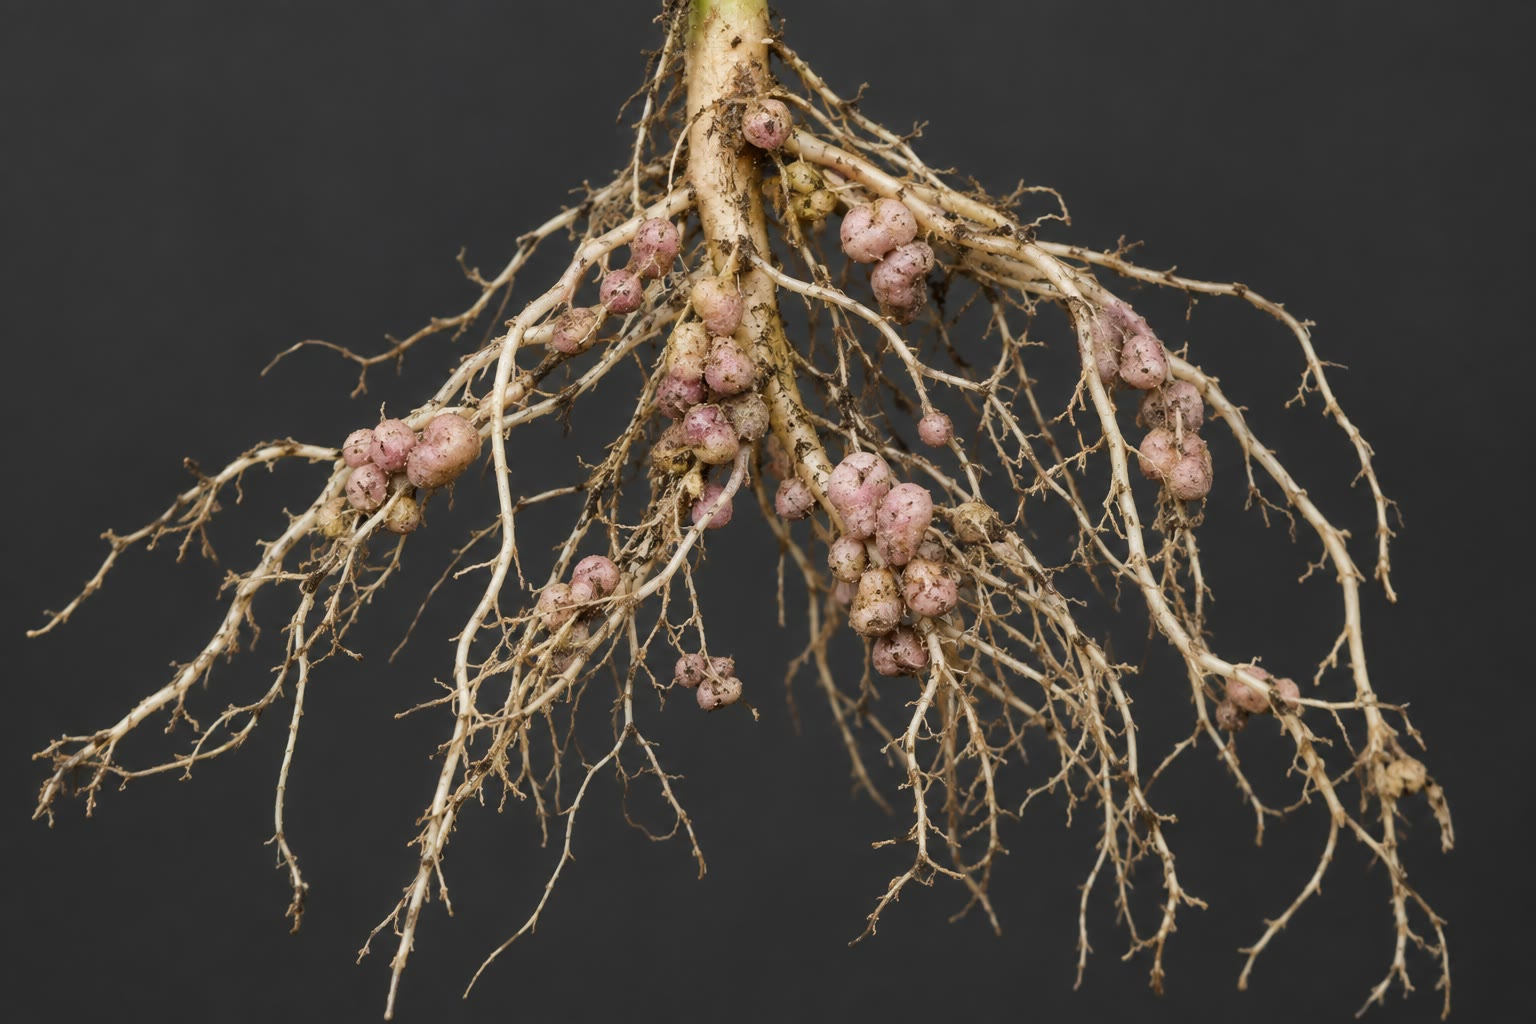
\includegraphics[width=0.44\linewidth]{images/book4/ai/b4-25-root-nodules.jpg}\hspace{0.04\linewidth}
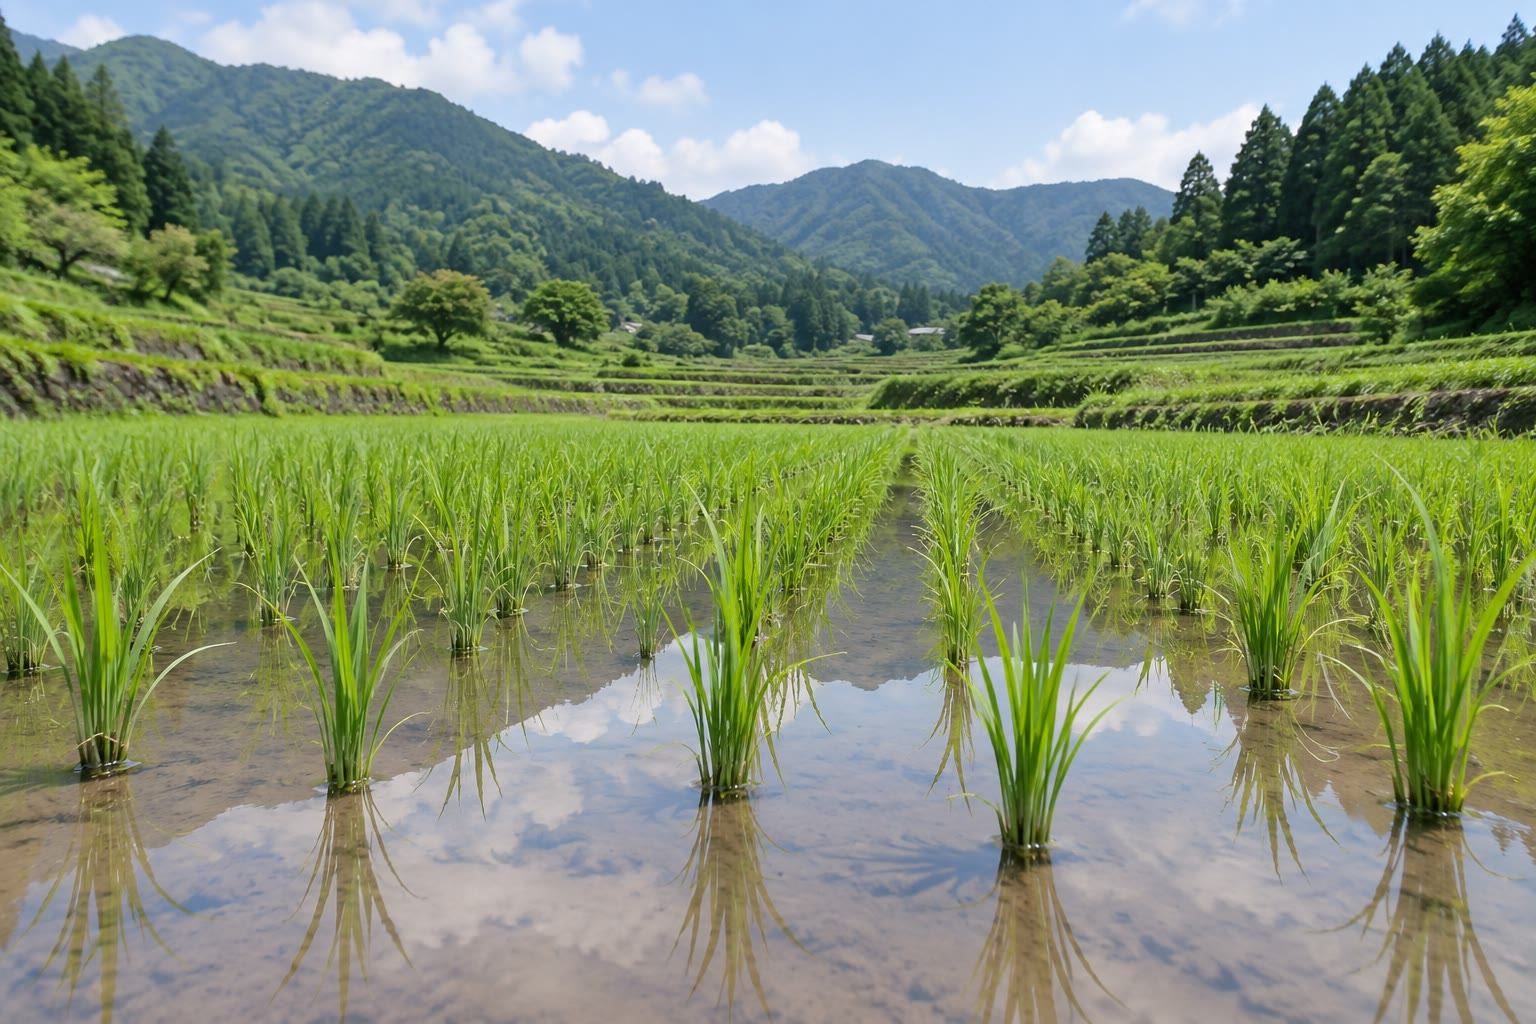
\includegraphics[width=0.44\linewidth]{images/book4/ai/b4-25-rice-paddy.jpg}

{\small Deux portes du \omterm{prop:b2:biogeochemical-cycles:nitrogen}{cycle de l'azote}. À gauche~: les nodosités
racinaires d'une légumineuse, chacune une chambre où des rhizobiums
fixent l'azote pour leur hôte. À droite~: une rizière inondée, anoxique
sous la surface, où la \omterm{def:b2:microbial-metabolism:anaerobic}{dénitrification} restitue l'azote à l'air et où les
méthanogènes fabriquent du méthane.}
\end{omfigure}

\section{La planète perturbée}

\begin{example}[Ce que disent les chiffres]\label{ex:b2:biogeochemical-cycles:numbers}
Des émissions de \qty{10}{GtC} par an avec une \omterm{prop:b2:biogeochemical-cycles:carbon}{fraction atmosphérique} de
$0.45$ laissent chaque année \qty{4.5}{GtC}, soit \qty{2.1}{ppm}, dans
l'air
--- la pente observée. Les émissions cumulées depuis 1850 atteignent
environ \qty{700}{GtC}, dont \qty{290}{GtC} se trouvent dans l'air
(140~ppm), le reste dans l'océan et les terres. Pour stabiliser
l'atmosphère à un niveau quelconque, les émissions nettes doivent tomber
à ce que les puits lents --- mélange avec l'océan profond et altération,
ensemble moins de \qty{1}{GtC} par an --- peuvent absorber~: la
\emph{neutralité carbone} n'est pas un slogan mais la condition d'\omterm{def:b2:biogeochemical-cycles:reservoir}{état
stationnaire} du \omterm{thm:b2:biogeochemical-cycles:box}{modèle à un compartiment} avec un $\tau$ très long. Pour
l'azote, le doublement du \omterm{def:b2:biogeochemical-cycles:reservoir}{flux} d'azote fixé a doublé le nitrate des
rivières, créé des zones mortes à l'embouchure du Mississippi et dans la
Baltique, et accru d'un cinquième le $\mathrm{N_2O}$ de l'atmosphère, un gaz à
effet de serre dont le \omterm{def:b2:biogeochemical-cycles:reservoir}{temps de résidence} est d'un siècle. Le
\cref{ch:b2:global-change} suit les conséquences pour les êtres vivants.
\end{example}

\section{Exercices}

\begin{exercise}[$\star$]\label{exo:b2:biogeochemical-cycles:1}
Définir \omterm{def:b2:biogeochemical-cycles:reservoir}{réservoir}, \omterm{def:b2:biogeochemical-cycles:reservoir}{flux} et \omterm{def:b2:biogeochemical-cycles:reservoir}{temps de résidence}, et calculer le \omterm{def:b2:biogeochemical-cycles:reservoir}{temps de
résidence} du carbone dans les plantes terrestres (450 GtC, photosynthèse
120 GtC par an) et dans l'océan profond (\num{37000} GtC, échange
d'environ 100 GtC par an).
\end{exercise}

\begin{exercise}[$\star$]\label{exo:b2:biogeochemical-cycles:2}
Convertir \qty{2.5}{ppm} par an en GtC, et \qty{10}{GtC} d'émissions en
ppm.
\end{exercise}

\begin{exercise}[$\star$]\label{exo:b2:biogeochemical-cycles:3}
Nommer les deux processus naturels qui ouvrent $\mathrm{N_2}$, le processus
qui le restitue, et les trois étapes d'oxydoréduction intermédiaires,
avec les organismes responsables.
\end{exercise}

\begin{exercise}[$\star$]\label{exo:b2:biogeochemical-cycles:4}
Pourquoi le phosphore limite-t-il la productivité plus souvent que l'azote
à l'échelle des temps géologiques, et l'azote plus souvent que le
phosphore au cours d'une saison donnée~?
\end{exercise}

\begin{exercise}[$\star\star$]\label{exo:b2:biogeochemical-cycles:5}
Un lac de \qty{e7}{m^3} reçoit \qty{2}{t} de phosphore par an et
renouvelle \qty{20}{\%} de son eau chaque année. Calculer sa concentration
en phosphore à l'\omterm{def:b2:biogeochemical-cycles:reservoir}{état stationnaire} et le temps nécessaire pour en
atteindre \qty{90}{\%} après le début de l'apport. Et si l'apport est
divisé par deux~?
\end{exercise}

\begin{exercise}[$\star\star$]\label{exo:b2:biogeochemical-cycles:6}
À partir des données de Keeling, calculer le taux de croissance moyen du
$\mathrm{CO_2}$ dans les années 1960 (de 316 à \qty{325}{ppm} en dix ans) et
dans les années 2010 (de 390 à 411 en neuf ans), en ppm par an et en GtC
par an.
\end{exercise}

\begin{exercise}[$\star\star$]\label{exo:b2:biogeochemical-cycles:7}
Les dents de scie saisonnières au Mauna Loa ont une amplitude d'environ
\qty{6}{ppm} du maximum au minimum. Convertir en GtC et comparer à la
production primaire nette annuelle des terres de l'hémisphère nord,
environ \qty{35}{GtC}. Pourquoi les dents de scie sont-elles tellement
plus petites~?
\end{exercise}

\begin{exercise}[$\star\star$]\label{exo:b2:biogeochemical-cycles:8}
La nitrogénase dépense 16 ATP par $\mathrm{N_2}$. Pour une légumineuse
fixant \qty{200}{kg} d'azote par hectare et par an, calculer le nombre de
moles de $\mathrm{N_2}$ fixées et l'ATP dépensé, et la masse de glucose que
représente cet ATP (environ 30 ATP par glucose). Quelle fraction des
photosynthétats d'une culture de \qty{10}{t/ha} cela représente-t-il~?
\end{exercise}

\begin{exercise}[$\star\star$]\label{exo:b2:biogeochemical-cycles:9}
Le plancton croît selon le rapport de Redfield $\mathrm{C:N:P} = 106:16:1$.
L'eau de mer profonde contient \qty{2.2}{\micro mol/kg} de phosphate et
\qty{32}{\micro mol/kg} de nitrate. Lequel s'épuise le premier lorsqu'une
masse d'eau est ramenée en surface, et quelle quantité de carbone est
fixée avant cet épuisement~?
\end{exercise}

\begin{exercise}[$\star\star\star$]\label{exo:b2:biogeochemical-cycles:10}
Traiter l'atmosphère comme un compartiment dont l'excédent de carbone $E$
est éliminé à la vitesse $E/\tau$ par les puits et alimenté par les
émissions $Q$. Avec $\tau =
50$ ans et $Q = \qty{10}{GtC/yr}$, quel est l'excédent à l'\omterm{def:b2:biogeochemical-cycles:reservoir}{état
stationnaire}, et à quelle concentration en ppm correspond-il~? Expliquer
pourquoi la réponse réelle est pire.
\end{exercise}

\begin{exercise}[$\star\star\star$]\label{exo:b2:biogeochemical-cycles:11}
Les essais nucléaires ont doublé le $\mathrm{{}^{14}C}$ de l'atmosphère en
1963~; l'excédent a ensuite diminué de moitié tous les 11 ans environ,
alors que le $\mathrm{{}^{14}C}$
a une demi-vie de 5730 ans. Expliquer ce qui a été mesuré, et ce que ces
11 ans nous apprennent sur le \omterm{prop:b2:biogeochemical-cycles:carbon}{cycle du carbone}.
\end{exercise}

\begin{exercise}[$\star\star\star$]\label{exo:b2:biogeochemical-cycles:12}
«~L'humanité a doublé le \omterm{prop:b2:biogeochemical-cycles:nitrogen}{cycle de l'azote} et n'a fait qu'effleurer le
\omterm{prop:b2:biogeochemical-cycles:carbon}{cycle du carbone}.~» Discuter chiffres à l'appui~: \omterm{def:b2:biogeochemical-cycles:reservoir}{flux} fixés, fractions
du \omterm{def:b2:biogeochemical-cycles:reservoir}{flux} naturel, et \omterm{def:b2:biogeochemical-cycles:reservoir}{réservoirs} touchés.
\end{exercise}

\section{Problème~: le bilan carbone d'un siècle}

\begin{problem}[{Problème du week-end --- un siècle d'émissions passé au
crible du modèle à un compartiment de l'atmosphère, la part de l'océan et
celle des terres, la cascade de l'azote d'un champ fertilisé à une zone
morte, et le bilan du phosphore d'un lac, jusqu'à la fraction
atmosphérique, à la concentration atmosphérique en 2100 et à l'azote
perdu par hectare}]
\label{pb:b2:biogeochemical-cycles:1}
Données. Atmosphère en 1850~: \qty{285}{ppm}~; \qty{1}{ppm} $=
\qty{2.13}{GtC}$. Émissions cumulées 1850--2020~: \qty{700}{GtC}~;
$\mathrm{CO_2}$ atmosphérique en 2020~: \qty{412}{ppm}. Un champ de
\qty{1}{ha} reçoit \qty{150}{kg} d'engrais azoté par an~; la culture en
absorbe \qty{60}{\%}, \qty{25}{\%} sont dénitrifiés, le reste est
lessivé. Un lac de \qty{5e7}{m^3} renouvelle un dixième de son eau par an
et reçoit \qty{5}{t} de phosphore par an.

\medskip
\noindent\textbf{Partie I --- La \omterm{prop:b2:biogeochemical-cycles:carbon}{fraction atmosphérique}.}
\begin{enumerate}
  \item Calculer le carbone atmosphérique en 1850 et en 2020, et
        l'augmentation en GtC.
  \item Calculer la \omterm{prop:b2:biogeochemical-cycles:carbon}{fraction atmosphérique} sur 1850--2020.
  \item Où se trouve le reste~? Donner les deux puits et, d'après la
        proposition, leurs parts approximatives.
  \item Si l'océan a absorbé \qty{25}{\%} des émissions, de combien son
        carbone inorganique dissous, \qty{38000}{GtC}, a-t-il augmenté en
        valeur relative~? Pourquoi l'océan superficiel s'acidifie-t-il
        néanmoins de façon mesurable~?
  \item Pourquoi la \omterm{prop:b2:biogeochemical-cycles:carbon}{fraction atmosphérique} reste-t-elle à peu près
        constante alors que les émissions croissent exponentiellement~?
        (Considérer le \omterm{thm:b2:biogeochemical-cycles:box}{modèle à un compartiment} avec
        $Q \propto e^{t/T}$ et un puits $E/\tau$.)
  \item Que deviendrait la \omterm{prop:b2:biogeochemical-cycles:carbon}{fraction atmosphérique} si les émissions
        restaient constantes pendant de nombreux siècles~?
\end{enumerate}

\medskip
\noindent\textbf{Partie II --- Le siècle à venir.}
Modéliser l'excédent de carbone $E$ (au-dessus du niveau de 1850) par
$\mathrm{d}E/\mathrm{d}t = Q - E/\tau$, $\tau = 100$ ans.
\begin{enumerate}[resume]
  \item Calculer l'excédent en 2020, en GtC.
  \item Avec $Q$ maintenu à \qty{10}{GtC/yr}, calculer l'excédent à l'\omterm{def:b2:biogeochemical-cycles:reservoir}{état
        stationnaire} et la concentration qu'il implique.
  \item Résoudre $E(t)$ à partir de 2020 avec $Q = 10$ et donner $E$ en
        2100 ainsi que la concentration.
  \item On fait maintenant décroître $Q$ linéairement jusqu'à zéro entre
        2020 et 2070, puis on le maintient à zéro. Calculer $E$ en 2070
        (intégrer l'équation~; la solution particulière pour un $Q$
        linéaire est une fonction affine) et en 2100.
  \item Comparer les deux concentrations en 2100.
  \item Pourquoi un $\tau$ unique est-il optimiste pour le second
        scénario~?
\end{enumerate}

\medskip
\noindent\textbf{Partie III --- La cascade de l'azote.}
\begin{enumerate}[resume]
  \item Calculer l'azote absorbé par la culture, dénitrifié et
        lessivé, par hectare et par an.
  \item L'azote lessivé atteint une rivière sous forme de nitrate, puis
        la mer, où le plancton l'utilise selon le rapport de Redfield.
        Quelle quantité de carbone permet-il au plancton de fixer~?
  \item Ce carbone sédimente et est respiré en profondeur, consommant de
        l'oxygène à raison d'un $\mathrm{O_2}$ par C. Calculer l'oxygène
        consommé, en moles et en kilogrammes.
  \item Un mètre cube d'eau de mer contient environ \qty{0.25}{mol} de
        $\mathrm{O_2}$ à saturation. Combien de mètres cubes d'eau de fond
        le lessivage d'un hectare désoxygène-t-il~?
  \item La fraction dénitrifiée s'échappe en partie sous forme de $\mathrm{N_2O}$,
        à raison de \qty{1}{\%} de l'azote dénitrifié. Calculer le $\mathrm{N_2O}$
        émis par hectare et par an, et son équivalent de réchauffement en $\mathrm{CO_2}$
        ($\mathrm{N_2O}$ vaut 270 fois $\mathrm{CO_2}$ par kilogramme).
  \item Comparer au $\mathrm{CO_2}$ émis pour fabriquer l'engrais
        (environ \qty{4}{kg} de $\mathrm{CO_2}$ par kilogramme d'azote par
        le \omterm{prop:b2:biogeochemical-cycles:nitrogen}{procédé Haber--Bosch}).
\end{enumerate}

\medskip
\noindent\textbf{Partie IV --- Le lac.}
\begin{enumerate}[resume]
  \item Calculer le \omterm{def:b2:biogeochemical-cycles:reservoir}{temps de résidence} du phosphore dans le lac si la
        seule perte est le renouvellement de l'eau, et sa concentration à
        l'\omterm{def:b2:biogeochemical-cycles:reservoir}{état stationnaire} en \unit{mg/m^3}.
  \item Les lacs contenant plus de \qty{30}{mg/m^3} de phosphore sont
        eutrophes. Celui-ci l'est-il~?
  \item La sédimentation élimine le phosphore avec sa propre constante de
        temps de 5 ans. Recalculer le \omterm{def:b2:biogeochemical-cycles:reservoir}{temps de résidence} et la
        concentration.
  \item L'apport est ramené à \qty{1}{t} par an. Calculer le nouvel \omterm{def:b2:biogeochemical-cycles:reservoir}{état
        stationnaire} et le temps nécessaire pour s'en approcher à moins de
        \qty{10}{\%}.
  \item Pourquoi de nombreux lacs se rétablissent-ils plus lentement que ne
        le prévoit ce calcul~?
  \item Calculer le carbone que le phosphore du lac peut incorporer
        chaque année au plancton selon le rapport de Redfield, à partir de
        l'apport de \qty{5}{t}.
  \item Énoncer le résultat~: la \omterm{prop:b2:biogeochemical-cycles:carbon}{fraction atmosphérique}, les deux
        concentrations en 2100, et l'azote lessivé par hectare.
\end{enumerate}
\end{problem}
